\chapter{Methodology}
    This chapter describes the series of procedures that was done to perform the study \textemdash from setting up the application, gathering data, creating the actual model and performing post-processing. It also states the technologies involved in the procedures. Furthermore, it explains the reasons and justifications for following such procedures and using such technologies.
\section{Application Development}
    The application was developed using Django, a Python-based Web framework. More specifically, the application is built atop GeoDjango, a module in Django that turns it into multi-featured GIS Web framework. This allows the creation and manipulation of spatially-enabled data especially that the application is dealing with city boundaries, crime locations and grids.

    The application's database backend is PostGIS, an extension of the PostgreSQL database. This kind of database adds support for geographic data and geometric objects allowing location and topographical queries to be run in SQL. This is the most recommended database backend for GIS applications because it has the best compatibility and support for GeoDjango.

    Through the features and functionalities provided by GeoDjango and PostGIS, we can handle criminal records, city boundaries and grids with ease. They can be represented as geometry objects such as points and polygons that we can easily create, store and fetch from the database using standard Python conventions. These geometry objects are wrapped with methods for handling coordinates, topology, projections and relations with other geometry objects. In the case of our application, a criminal record has an attribute that contains a point, representing the location (latitude, longitude) where the incident happened. This point contains a method that can check if it is on a given cell of a grid, which is represented by a polygon object.

\section{Datasets}
    \subsection{City Boundaries}
        The data for the boundaries of Chicago City was downloaded from the city's official data portal at data.cityofchicago.org. The downloaded file is of zip format containing the different shape files representing the data for the city boundaries. The data was imported to the database via GeoDjango's LayerMapping data import utility (see Appendix \ref{code-loadmap}). The boundary of Chicago city are saved in the database as a CityBorder model instance (see Appendix \ref{code-cityborder}). 
    \subsection{Criminal Records}
        The criminal records of Chicago are from their dataset that is also in the city's data portal. The dataset can be accessed using the Socrata Open Data API (SODA). The criminal records were fetched and saved in the database via SodaPy (see Appendix \ref{code-fetchcrimes}), a package that binds SODA with Python. These records are represented by the CriminalRecord model. The criminal records in the dataset spans from January 1, 2001 to March 24, 2016. Though the dataset is frequently updated, this study used the criminal records within that given period. These criminal records are represented in the database as CriminalRecord model instances (see \ref{code-criminalrecord}).

\section{Generating the Grid}
    \begin{figure}[H]
    \centering
    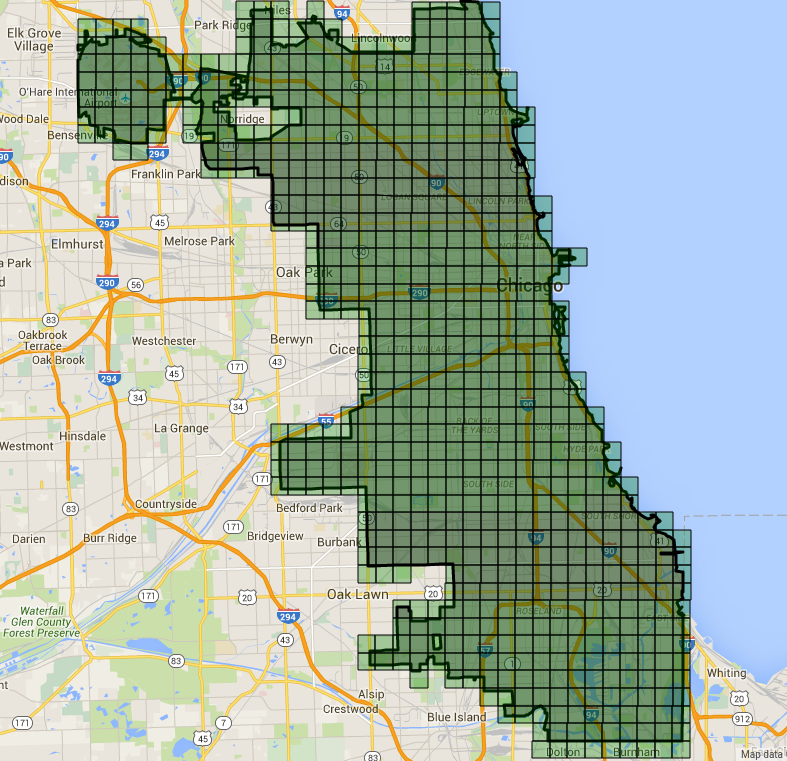
\includegraphics[width=12cm]{grid-example}
    \caption{An example of a grid.}
    \label{fig:grid}
    \end{figure}
    The map grid is created using a series of GeoDjango methods. GeoDjango's geometry objects, such as Polygon and Point, are wrapped with the GEOS (Geometry Engine - Open Source) API. The GEOS API implements SQL spatial functions and operators that allows us to create geometry objects and perform operations and comparisons between location, area and length of objects. However, GeoDjango lacks the support for geodetic functions to deal with distances with respect to the spherical nature of the Earth. Distances cannot be handled linearly and the curvature of the Earth must be taken into consideration. To support this, a library called GeoPy is used. Figure \ref{fig:grid} shows an example of the generated grid.

    The grid is generated as a list of boxes with dimension based on the given size. The envelope of the city boundary, represented as a polygon object, is determined as the largest quadrilateral that encapsulates all points of the boundary. The northwest point of this envelope is obtained and used as starting point to generate the cells of the grid. A cell will be created by calculating the other vertices of the box along with the starting point depending on the given dimension. The cell will only be included to the grid when it intersects the boundary of the city. The starting point for the next box will be the top-right corner of the newly created cell. This will continue until a whole row is completed. The next cell will then be generated in the next row. This process is repeated until the whole city area is covered. The list of cells which represents the grid will be saved in a pickle file so that the grid will be easily fetched next time instead of performing the calculations again. The code for generating the grid can be seen in Appendix \ref{code-cityborder} under the method name \textit{generateGrid}.

\section{Data Collection and Preprocessing}
    The input data for our learning model is a sequence of periodic snapshots by week, month or year of the presence or absence of a crime type per cell. A row of data has the same number of entries as the number of cells in the grid. For each cell in the grid, CriminalRecord objects are fetched and filtered as to which records happened within the boundaries of that cell for the given crime type. If no crime type is given, all types of crime will be considered. If there is a crime in that cell, the corresponding index in the row of data will have 1. If none, -1 will be entered. So, a row of data is a series of 1 or -1 that corresponds to the presence or absence of a crime type in each grid. This will be repeated for each year, month or week. So the final data is a 2-dimensional array of different months, years or weeks, each of which has a row of data for each grid.

    For seasonal data, a row of input is another 2-dimensional array that contains the grid snapshots of crime incidents for different seasons of a period. A season is defined to be the same week or month for different years. So a seasonal input has multiple rows for each week, month or daily period, each of which contains the different snapshots for that wee or month on different years.

    The code followed for data vectorization can be seen in Appendix \ref{code-vectorization}.

\section{Machine Learning Model}
    The learning model used is built using a library called Keras because it implements the original LSTM proposed by Hochreiter and Schmidhuber \citeyearpar{hochreiter1997long}. The input of the model is the sequence of periodic snapshots of the states of each cell in the grid obtained during data preprocessing. It is divided into training and test sets with 0.7 ratio. The model contains a layer of LSTM cells, one for each input in the data. The model's training is done through 1000 epochs.

    The code for running the LSTM network is in Appendix \ref{code-network}.

\section{Experiments}
    A set of experiments were done to evaluate the performance of the model under different conditions and parameters. The parameters that are being experimented upon are the cell dimensions of the grid, period of snapshots and the implementation of crime seasonality. The results of these experiments are measured through certain performance metrics in order to determine the effectiveness of the model.

\section{Performance Metrics}
    To measure the performance of the model, several performance metrics is implemented. The Mean Squared Error (MSE) is used to measure the error of the predicted output values with respect to the target values. Accuracy and F1 Score values is used to measure the accuracy of the model when predicting the next state of the cells in the grid.

\section{Error Analysis}
    The performance of the model is then evaluated through error analysis. Learning curves are plotted showing the training error and cross-validation error of the model using different training sample sizes. The graphs will be generated using Scikit Learn's \textit{learning\_curve} method results plotted using matplotlib. The cross-validation technique is k-fold cross-validation using three folds. The error measured in the graphs is the MSE.

    The code for running the error analysis is in Appendix \ref{code-error-analysis}.
